\section{Replacing \code{foreach} loops with \code{for} loops}

In Java, the \code{for} statement\footnote{\url{https://docs.oracle.com/javase/specs/jls/se8/html/jls-14.html#jls-14.14}}
has two forms: the basic one and the enhanced one. Since the meaning of the enhanced \code{for} statement is given by
translation into a basic \code{for} statement\footnote{\url{https://docs.oracle.com/javase/specs/jls/se8/html/jls-14.html#jls-14.14.2}},
the enhanced form is merely syntactic sugar for the basic one.

This pass first collects all the enhanced \code{for} statements in the method body which contain at least one recursive
call in pre-order fashion by using a visitor processing children nodes before the current node. Then it replaces these
statements by their equivalent basic \code{for} statements. This conversion is necessary because control flow needs to
be explicit for later stages in the refactoring process. The \textit{Condition} and \textit{Update} parts of a \code{for}
statement in particular need to be explicit because they get executed after returning from a recursive call in the body
of the \code{for} statement.

There are two cases for this conversion: the first when the type of \textit{Expression} is a subtype of
\code{Iterable} (exemplified in \labelindexref{Figure}{img:foreach-to-iterator-for}) and the second when
\textit{Expression} has an array type \code{T[]} (exemplified in \labelindexref{Figure}{img:foreach-to-indexed-for}),
where \textit{Expression} is the value over which the enhanced \code{for} statement iterates.

\begin{figure}[htb]
    \makebox[\linewidth][c]{%
    \begin{subfigure}[b]{.5\textwidth}
        \centering
        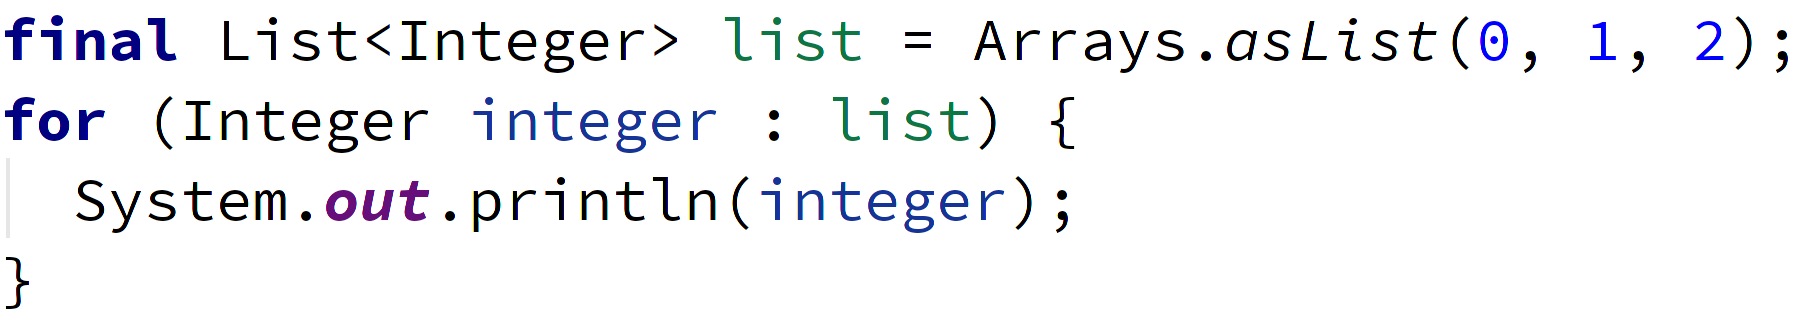
\includegraphics[height=0.5in]{src/img/foreach-to-iterator-for-before-white.png}
        \caption{Before}
    \end{subfigure}%
    \begin{subfigure}[b]{.5\textwidth}
        \centering
        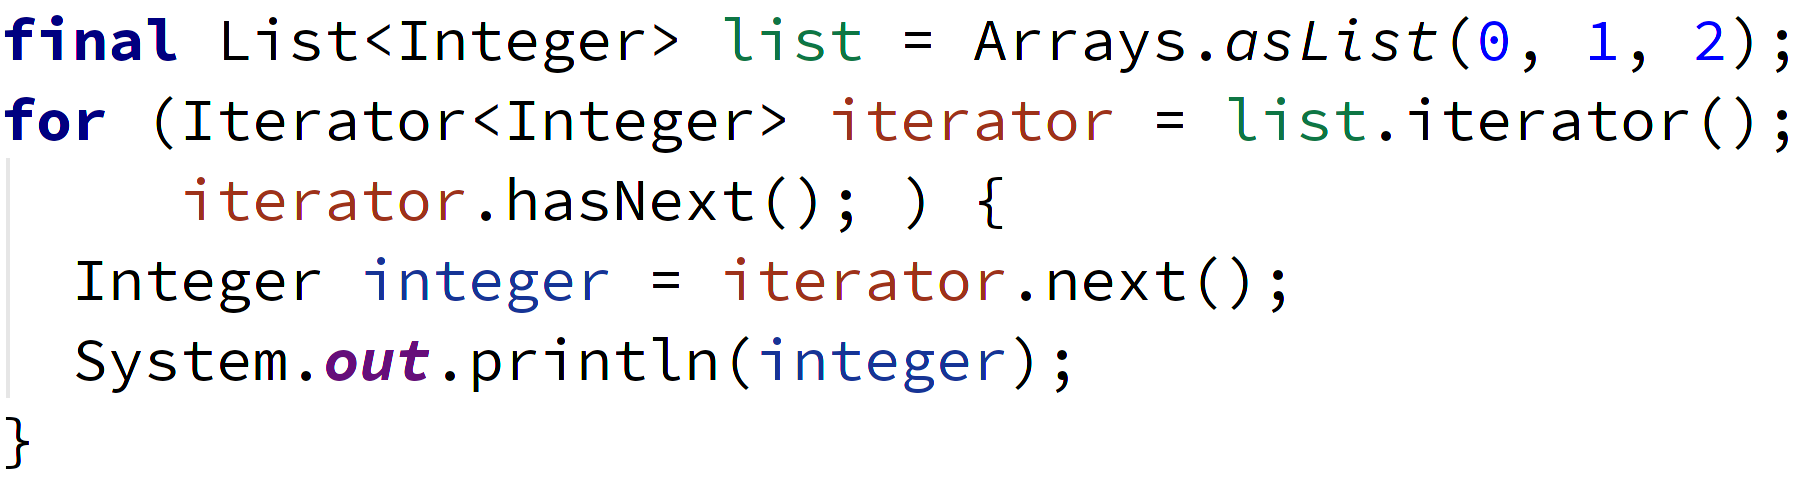
\includegraphics[height=0.75in]{src/img/foreach-to-iterator-for-after-white.png}
        \caption{After}
    \end{subfigure}%
    }\\
    \caption{\code{Foreach} loop to iterator \code{for} loop conversion \label{img:foreach-to-iterator-for}}
\end{figure}

\begin{figure}[htb]
    \makebox[\linewidth][c]{%
    \begin{subfigure}[b]{.5\textwidth}
        \centering
        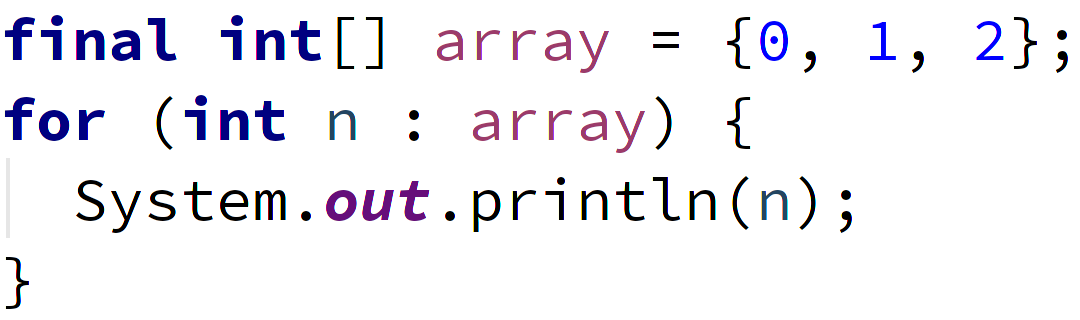
\includegraphics[height=0.5in]{src/img/foreach-to-indexed-for-before-white.png}
        \caption{Before}
    \end{subfigure}%
    \begin{subfigure}[b]{.5\textwidth}
        \centering
        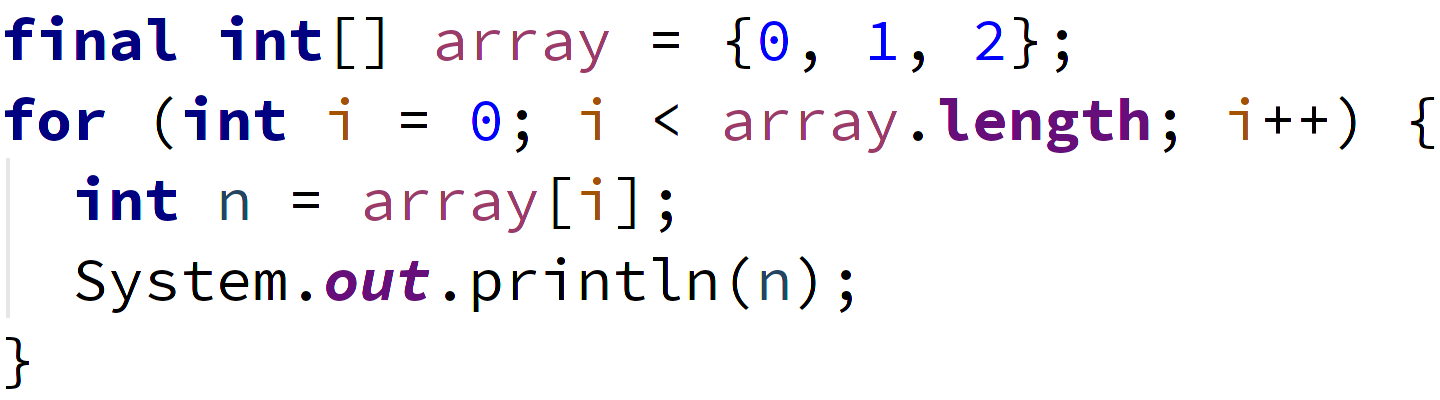
\includegraphics[height=0.625in]{src/img/foreach-to-indexed-for-after-white.png}
        \caption{After}
    \end{subfigure}%
    }\\
    \caption{\code{Foreach} loop to indexed \code{for} loop conversion \label{img:foreach-to-indexed-for}}
\end{figure}
